\documentclass[journal]{IEEEtran}

\usepackage{blindtext}
\usepackage{cite}
\usepackage{graphicx}
\usepackage{array}
\usepackage{color}
\usepackage{tabularx}
\usepackage{epsfig}
\usepackage{amsmath}
\usepackage{amssymb}
\usepackage{bm}
\usepackage{wasysym}
\usepackage{circuitikz}
\usepackage{float}
\usetikzlibrary{arrows,shapes,calc,positioning}

\newcommand{\myscope}[2]
{\draw[thick,rotate=#2] (#1) circle (12pt)
(#1) ++(-0.35,-0.1) --++ (0.3,0.3) --++ (0,-0.3) --++(0.3,0.3) --++(0,-0.3);}

\begin{document}

\title{CSCE 221 \\ Problem Set 3}

\author{Jacob~Purcell,~\IEEEmember{Texas~A\&M,~Student}}

\maketitle
\section{}
\subsection*{a}

Procedure in "printLots.h".

\subsection*{b}

Assuming a datastructure that returns at() with $O(1)$, printLots() is $\boxed{O(N)}$. at() may also
iterate through the entire vector up to the needed index in which case printLots() is $O(N^2)$.


\section{}

\subsection*{a}
Procedure in "intersection.h".

\subsection*{b}
Okay.

\subsection*{c}
intersection() is a for loop of one vector<int> nested in another for loop for another vector<int>. Since 
they are combined in such a way that runs $N$ times $N$ times (for each increment of $N$, the Procedure 
will iterate $N$ more times) the procedure runs at $O(N^2)$. 

\section{}

\subsection*{a}
Procedure in "josephus.h".

\subsection*{b}

The first pass requires $N$ computations, the second pass requires $N - \frac{N}{2}$, the third pass will then require
$(N - \frac{N}{2}) - \frac{N}{4}$ and so on. It seems that the number of computations goes as 

$$f(N) = (\Sigma_{i=0}^{I = N} \frac{N}{-2^i})$$

When $i = N$, the final element has been found and the $\Sigma$ terminates. It can be seen that this series is geometric 
and convergent $\forall N \cdot M \epsilon $. $f(N)$ is a linear combination of computations, the volume of which decays as 
$\frac{1}{2^i}$. Higher order terms are quickly dominated by the first term and as such, 
$O(f(N)) = \boxed{O(N)}$. 


\subsection*{c}

\subsubsection{1}

As seen in Fig. 1, garbage collection takes up most of the computation time, however, still grows as $O(N)$. Since 
garbage collection and computation differ only by a constant, as $N \rightarrow \infty$, the 3 series are identical.
However, all nontrivial datasets are finite and it would still be desireable to minimise the prevalence of the garbage 
collection step, and complete the computations in a fraction of the time (out most precious resource). An immediate 
solution would be to move reduce the problem from an iterative problem to a pure math problem, which would bring the 
computational time down to $O(1)$ with no need for garbage collection. I suspect that a function of $N$ and 
$M$ will produce the winner without the need for creating a large list. My initial investigation leads me to beleive that the winner is chosen with 
periodicity $\tau(N,M)$. I ran the algorithm for this problem to tell me the results and the winnder does indeed follow
a periodic pattern that grows every reset. Unfortunately, I am unable to follow this to it's conclusion due to time constraints, 
however, the first $10k$ winners are found in "win.txt".

In every chart, anomalous spikes and noise stem from cpu multitasking and temperature change. Fig. 1 shows an 
area of low noise and high precision, this is just the result of leaving my computer running at night.

\begin{figure}[h!]
	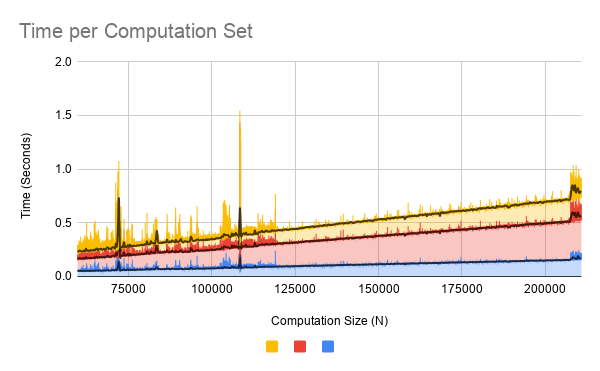
\includegraphics[scale = 0.5]{TC1.png}
	\caption{Yellow: Total computation time, Red: Time taken by data management to allocate and deallocate 
            space for N people, Blue: Time needed to compute the winner for a given N.}
\end{figure}


\subsubsection{2}

Black trendline represents the moving average of the elimination step, which decays exponentially for a given N. The sudden spikes are a new 
list, and each subsequent iteration follows $f(N)$ as previously discussed. As such, the overall computation time 
for each iteration goes as $O(N)$. As seen in Fig. 3, the behaviour of the elimination step becomes more apparent for large ($200k$) values of N. 
Unfortunately I am not able to plot every collected datapoint ($7M$) with excel or google to 
show asymptotic behaviour (it seems to be constant but it is suspected that the view is 
too small to get an accurate depiction). Right now I am trying to figure out an efficient 
way of plotting such datasets. As it stands, this chart still goes as $O(N)$. 

\begin{figure}[h!]
	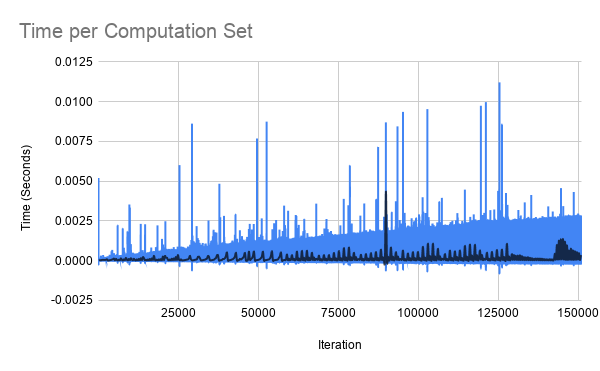
\includegraphics[scale = 0.5]{TC2.png}
	\caption{This chart shows initial growth of iterations as N grows.}
\end{figure}

\begin{figure}[h!]
	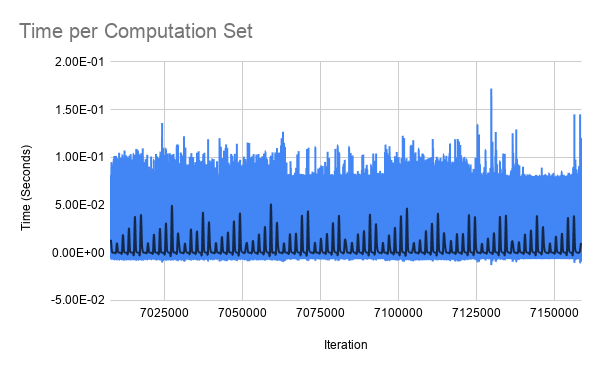
\includegraphics[scale = 0.5]{TC3.png}
	\caption{Elimination time for large values of N ($200k$).}
\end{figure}



\end{document}
